% !TeX spellcheck = nl_NL
\documentclass{article}

\begin{document}
	\section{Data-service}
	
	\subsection{De Service}
	Om onze databank aan te spreken gaan we een rest service voorzien waar we enkele simplistische methodes toekennen die het mogelijk maken om: de ids van de gewijzigde data periodiek op te halen aan de hand van een datum die fungeert als ondergrens en een endpoint waar we één element kunnen ophalen aan de hand van een id. Dit maakt het mogelijk om via een schedular systematisch de gewijzigde producten, winkels en prijzen uit onze databank op te halen en naar AEM te versturen. Of dat dit effectief de beste plan aanpak is voor onze drie modellen kunnen we later nog herzien en, indien dit niet het geval is, onze service aanpassen.
	\par
We gebruiken hiervoor een Java Spring-boot service omdat deze makkelijk in opzet zijn maar gezien het een rest service is kan hier perfect voor een andere programmeertaal gekozen worden. Onze configuratie zullen we doen via een application.yml bestand, deze wordt automatisch door de laatste versie van Spring-boot ondersteund.
\par
Om te connecteren met onze Cassandra cluster maken we gebruik van de Datastax java-driver. Datastax is een bedrijf dat een commerciële versie van Apache Cassandra aanbiedt alsook support voorziet. Hun Java-driver is open-source en dus gratis te gebruiken, in mijn ervaring biedt deze ook een betere ondersteuning voor het gebruik van UDTs tegenover de JPA-implementatie voor Cassandra. Om deze driver te gebruiken moeten we onze klassen die overeenstemmen met een tabel in onze databank annoteren met ‘@Table’. De velden in deze klassen krijgen nog de annotatie ‘@Column’ en ‘@PartitionKey’ als het gaat om een primary key kolom. De types van onze databank voorzien we ook klassen voor die we annoteren met ‘@Field’. De velden hier annoteren we met ‘@Field’. Eenmaal we onze tabellen hebben vertaald naar overeenstemmende klassen volstaat het om een sessie met onze cluster aan te maken, bij het aanmaken hiervan volstaat het om het IP-adres van één node te voorzien, de driver zal dan via discovery de locatie van de overige nodes vinden en zo fouttolerantie te waarborgen. Het is toch aan te raden om meerdere IP-adressen mee te geven zodat wanneer er een node niet beschikbaar is tijdens het aangaan van de sessie, deze kan terugvallen op een andere node.
\par
Verder voorzien we drie rest controllers: één voor elk hoofdmodel dat we hebben voorzien. Voor onze AEM-applicatie te kunnen voeden moeten we minstens twee endpoints per controller moeten voorzien, één voor het ophalen van de gewijzigde IDs per model en één voor het effectief ophalen van de data. 
	\subsection{Docker}
	De volgende stap is ons process is een manier zoeken om onze service in de cloud te draaien. Het is aanvaardbaar om tijdens de ontwikkeling onze service lokaal te draaien maar als we een volwaardig platform willen creeeren moet ook dit onderdeel remote draaien.
	\par
	\begin{wrapfigure}{r}{0.5\textwidth}
  	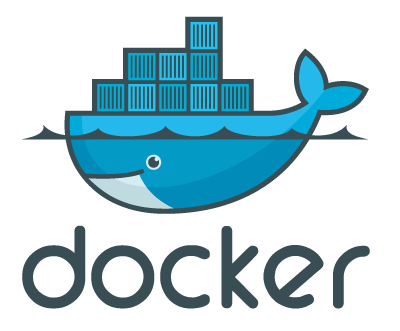
\includegraphics[width=0.4\textwidth]{images/docker-logo.PNG}
	\end{wrapfigure}
	
	Docker is een open-source project dat dit process voor ons zal versimpelen. Vroeger moest er heel wat tijd (en bijgevolg ook budget) gespendeerd worden aan het werkende krijgen van services op verschillende machines. Dit komt omdat niet elke machine hetzelfde geconfigureerd is alles even goed ondersteund. Docker lost dit probleem op door maar één vereiste te hebben, dat de machine de Docker service heeft draaien. Oorspronkelijk ondersteunde enkel Linux systemen deze service native maar ondertussen zijn ook Windows en Mac mee op de kar gesprongen. Om deze lokaal te trainen, voor testing doeleinden, kan men naar de docker website gaat en de gewenste versie te downloaden. De tutorials die je daar kan vinden leggen perfect uit hoe je ermee aan de slag kan. Natuurlijk gaan we, na een korte uitlichting, onze Docker remote gaan draaien.
	\par
	Wie Docker zegt, zegt containers. Om onafhankelijk van de host een applicatie te kunnen draaien, steekt Docker deze, en al het nodige (environment, tools, libraries,settings,...), in een container. Docker bundelt al het nodige samen en maakt er een exporteerbare image van. Deze image kunnen we dan eender waar draaien zonder ons zorgen te moeten maken om infrastructurelen verschillen. Dit wil zeggen dat wanneer een image succesvol in een trainingsomgeving draait, deze zonder vrees overgezet kan worden naar een productie omgevening.
	\par
	Een ander voordeel van het containersysteem is dat men elke container, tijdens het opstarten, specifieke parameters kan meegeven met betrekking tot de resources die deze ter beschikking krijgt. Als men enkele zwaardere services heeft, kan met de container hiervan meer RAM toekennen dan anderen om aan de behoefte te voldoen. Het is perfect mogelijk om meerdere containers op één machine of verdeelt over meerdere machines te draaien wat de schaalbaarheid en beschikbaarheid ten goede komt. Zelfs een release hoeft geen downtime meer te betekenen, de containers kunnen één voor één vervangen worden met een nieuwere versie.
	\subsection{AWS en Docker}
	Nu wordt het tijd dat we onze services naar onze AWS-cluster gaan draaien. Hiervoor zijn enkele stappen nodig begint bij de installatie van de nodige software op onze ontwikkelings machine. De eerste is de AWS Command Line Interface (of kortweg AWS CLI), gelukkig voor ons heeft Amazon hier een uitstekende handleiding\footnote{http://docs.aws.amazon.com/cli/latest/userguide/installing.html}
	voor. Het is belangrijk niet te vergeten om na de installatie deze ook te configureren\footnote{http://docs.aws.amazon.com/cli/latest/userguide/cli-chap-getting-started.html}.
	\par
	Het tweede wat we nodig zullen hebben is Docker op onze ontwikkelings machine, niet omdat we onze containers hier gaan draaien maar omdat we deze hier gaan bouwen. Voor diegene zonder ervaring met Docker raad ik deze manier aan om een beter begrip te krijgen van hoe dit in zijn werk gaat. De ervaren lezer mag natuurlijk zijn images op zijn gekozen manier bouwen. Om Docker te installeren kan de Linux-gebruiker zijn shell gebruiker, Mac en Windows hebben minder geluk en zullen een installer\footnote{https://docs.docker.com/engine/installation/} moeten gebruiken.
	\par
	Eenmaal onze ontwikkelings machine klaar is keren we terug naar AWS om een ECS (EC2 Container Service) op te zetten, hierin gaan we onze containers laten draaien. Een cluster kunnen we zien als een logische groepering van machines, wanneer we een containers deployen zullen deze automatisch verdeelt worden over deze machines.
	\par
	Voor we aan de slag gaan zullen we snel 2 IAM, één rol voor onze machines en één rol voor de service die we op onze cluster zullen starten. De rol voor de machines geven we een logische naam: ecs-instance-role en geven we de permissie AmazonEC2ContainerServiceforEC2Role {Geeft de machine schrijfrechten op CloudWatch en ECS, leesrechten op ECR}. De rol voor de service noemen we ecs-service-role en geven we de de permissie AmazonEC2ContainerServiceRole (schrijf-en leesrechten op EC2 en ELB). 
	\par	
	 Een ECS cluster opzetten is geen werk, even navigeren naar scherm, kiezen om een nieuwe te maken, we geven deze een naam(bv. tst-ecs-cluster) en voor nu selecteren we de optie 'Create an empty cluster'. Als we nu een cluster aanmaken dan zien we deze verschijnen onder cluster verschijnen maar zonder instances in, deze toevoegen is een volgende stap.
	\par
	Vervolgens maken we een Launch configuration aan, dit zal beschrijven hoe onze machines opgestart moeten worden. De configuratie heeft als voordeel dat we dit maar eenmaal moeten doen en dat alle machines binnen onze cluster met de zelfde configuratie opstarten. DIt is grotendeels gelijk aan het maken van een machine, let wel op dat als AMI\footnote{Amazon Machine Image} de Amazon ECS-optimized\footnote{te vinden onder AWS Marketplace} kiest. Dit zal onze services automatisch van Docker voorzien en deze ook starten wanneer de machine boot. Ken ook de ecs-instance-rol toe aan onze machines bij de stap Configure details. In deze stap voegen we ook een script toe onder User data (Advanced Details). Hier schrijven we het script als gezien in Figuur \ref{fig:ecs-script}. Dit zal ervoor zorgen dat onze machines beschikbaar zijn in onze cluster.
	\begin{figure}[h!]
		\centering
  		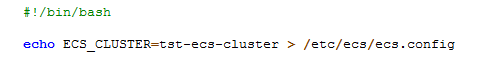
\includegraphics[width=0.5\textwidth]{images/ecs-script.PNG}
  		\caption{ECS bootup script.}
  		\label{fig:ecs-script}
	\end{figure}
	\par
	Nu we een Launch configuration hebben kunnen we deze gebruiken om effectief machines aan te maken.
\end{document}

